\documentclass[helvetica]{seminar} 
\input{xy}
\xyoption{all}
\usepackage{graphicx} 
\usepackage{slidesec} 
\usepackage{url}
\usepackage[framemethod=TikZ]{mdframed}
\usepackage{color}
\usepackage[normalem]{ulem}  

\def\dash---{\unskip\kern.16667em---\penalty\exhyphenpenalty\hskip.16667em\ignorespaces}
\long\def\symbolfootnote[#1]#2{\begingroup%
\def\thefootnote{\fnsymbol{footnote}}\footnote[#1]{#2}\endgroup}

% to fix problems making landscape seminar pdfs
% Letter...
\pdfpagewidth=11truein
\pdfpageheight=8.5truein
\pdfhorigin=1truein     % default value(?), but doesn't work without
\pdfvorigin=1truein     % default value(?), but doesn't work without
% A4
%\pdfpagewidth=297truemm % your milage may vary....
%\pdfpageheight=210truemm
%\pdfhorigin=1truein     % default value(?), but doesn't work without
%\pdfvorigin=1truein     % default value(?), but doesn't work without


\renewcommand{\familydefault}{\sfdefault}  
 
\input{seminar.bug} 
\input{seminar.bg2} % See the Seminar bugs list 
 
\slideframe{none} 
 
 
\usepackage{fancyhdr} 
 
% Headers and footers personalization using the `fancyhdr' package 
\fancyhf{} % Clear all fields 
\renewcommand{\headrulewidth}{0mm} 
\renewcommand{\footrulewidth}{0.1mm} 
 
\fancyfoot[L]{\tiny IETF 96} 
\fancyfoot[C]{\tiny TLS}
\fancyfoot[R]{\tiny \theslide} 
 
 
% To center horizontally the headers and footers (see seminar.bug) 
\renewcommand{\headwidth}{\textwidth} 

% To adjust the frame length to the header and footer ones 
\autoslidemarginstrue 
\pagestyle{fancy} 
 

\newcommand{\heading}[1]{% 
  \begin{center} 
    \large\bf 
    #1 
  \end{center} 
  \vspace{.4 in}} 



\begin{document}

\begin{slide}
\begin{center}
\vspace{.5 in}
\LARGE{{\bf}TLS 1.3\\{\small \verb^draft-ietf-tls-tls13-14^}}\\
\vspace{.2in}
\large{
\begin{tabular}{c}
Eric Rescorla\\
Mozilla\\
\url{ekr@rtfm.com}
\end{tabular}
}
\end{center}
\end{slide}

\centerslidesfalse 

\begin{slide}
\heading{Major changes since draft-12}

\vspace{-8ex}
\begin{itemize}
\item Remove 0-RTT (EC)DHE and client auth
\item Complete 0-RTT PSK mode
\item Restructure key schedule
\item Add session context
\item Fully define HelloRetryRequest
\item NewSession ticket use flags
\item Allow server to send SupportedGroups
\item Move CertificateStatus to an extension
\item Add ticket age for anti-replay
\item Allow resumption after fatal alerts
\item Remove non-closure warning alerts
\item Add Security Analysis section
\end{itemize}

\end{slide}


\begin{slide}
\heading{0-RTT is now PSK-only}

\vspace{-3ex}
\begin{scriptsize}
\begin{verbatim}
            ClientHello
              + early_data
              + pre_shared_key
              + key_share*
            (Finished)
            (Application Data*)
            (end_of_early_data)       -------->
                                                            ServerHello
                                                           + early_data
                                                       + pre_shared_key
                                                           + key_share*
                                                  {EncryptedExtensions}
                                                  {CertificateRequest*}
                                                             {Finished}
                                      <--------     [Application Data*]
            {Certificate*}
            {CertificateVerify*}
            {Finished}                -------->
            [Application Data]        <------->      [Application Data]
\end{verbatim}
\end{scriptsize}
\end{slide}

\begin{slide}
\vspace{-8ex}
{\tiny
\begin{verbatim}
                 0
                 |
                 v
   PSK ->  HKDF-Extract
                 |              
                 v
           Early Secret  --> Derive-Secret(., "early traffic secret", ClientHello)
                 |                         = early_traffic_secret
                 v
(EC)DHE -> HKDF-Extract
                 |
                 v
              Handshake
               Secret -----> Derive-Secret(., "handshake traffic secret", ClientHello + ServerHello)
                 |                         = handshake_traffic_secret
                 v
      0 -> HKDF-Extract
                 |
                 v
            Master Secret
                 |
                 +---------> Derive-Secret(., "application traffic secret", ClientHello...Server Finished)
                 |                         = traffic_secret_0
                 |
                 +---------> Derive-Secret(., "exporter master secret", ClientHello...Client Finished)
                 |                         = exporter_secret
                 |
                 +---------> Derive-Secret(., "resumption master secret", ClientHello...Client Finished)
                                           = resumption_secret


\end{verbatim}
}
\end{slide}

\begin{slide}
\heading{Session Context}

\begin{itemize}
\item Multiple requests to include more context when resuming (Krawczyk, Bhargavan)
\end{itemize}

{\footnotesize
\begin{verbatim}
     resumption_psk = HKDF-Expand-Label(resumption_secret,
                                        "resumption psk", "", L)

     resumption_context = HKDF-Expand-Label(resumption_secret,
                                            "resumption context", "", L)
\end{verbatim}
}

\begin{itemize}
\item Merged into handshake hashes whenever used
\end{itemize}

{\footnotesize
\begin{verbatim}
     Hash(Messages) + Hash(resumption_context)
\end{verbatim}
}
\end{slide}


\begin{slide}
\heading{Cookies for HelloRetryRequest}

\begin{itemize}
\item Derived from DTLS (and originally Photuris)
\item Server can provide a cookie with HRR 
\item Client echoes it with new ClientHello
\item Usable for stateless reject by pickling the handshake state in the cookie
\end{itemize}
\end{slide}


\begin{slide}
\heading{Post-Handshake Key Separation}

\begin{itemize}
\item General consensus on list to leave as-is
\item Analysis from Hugo Krawczyk indicates this is OK
\item IMPORTANT: We still have key separation for handshake and app data.
\end{itemize}
\end{slide}


\begin{slide}
\heading{Cipher Suite Negotiation: Problem Statement}

\begin{itemize}
\item The cipher suite negotiation has gotten clunky and non-orthogonal
\item Already was bad in 1.2
  \begin{itemize}
  \item Cipher suite, signature algorithms, named groups
  \end{itemize}
\item Worse in 1.3 
  \begin{itemize}
  \item PSK, key shares
  \end{itemize}
\item Can we radically simplify?
\end{itemize}
\end{slide}

\begin{slide}
\heading{Cipher Suite Negotiation: Overview}

\begin{itemize}
\item Make things as orthogonal as possible
  \begin{itemize}
  \item AEAD-PRF
  \item Signature algorithms
  \item Key shares/named groups
  \item PSK
  \end{itemize}

\item Negotiate each separately
  \begin{itemize}
  \item Straightforward for public key
  \item PSK makes things a bit complicated
  \end{itemize}
\end{itemize}
\end{slide}

\begin{slide}
\heading{Public key algorithm negotiation}

\begin{itemize}
\item Cipher suite just indicates AEAD and PRF
  \begin{itemize}
  \item Probably define new cipher suites
  \item Added bonus of letting us prune!
  \end{itemize}

\item Signature algorithms determines server cert/key and signature scheme
\item Key shares and supported groups determine the key exchange
  \begin{itemize}
  \item Model everything as (EC)DHE
  \item Server's key share indicates which group it picked
  \end{itemize}
\end{itemize}
\end{slide}

\begin{slide}
\heading{What about PSK?}

\vspace{-5ex}
\begin{itemize}
\item PSK can be combined with (EC)DHE and signatures (new) (?)
\end{itemize}

\vspace{-1ex}
\begin{scriptsize}
\begin{verbatim}
    enum { psk_ke(0), psk_dhe_ke(1), (255) } PskKeModes;
    enum { psk_auth(0), psk_sign_auth(1), (255) } PskAuthModes;

    struct {
       PskAuthMode auth_modes<1..255>;
       PskKeMode ke_modes<1..255>;
       opaque identity<0..2^16-1>; 
    } PskIdentity;

    struct {
         select (Role) {
             case client:
                 PskIdentity identities<2..2^16-1>;
              case server:
                 PskAuthMode auth_mode;
                 PskKeMode ke_mode;
                 uint16 selected_identity;
         }
     } PreSharedKeyExtension;
\end{verbatim}
\end{scriptsize}
\end{slide}


\begin{slide}
\heading{Should we change negotiation?}

\begin{itemize}
\item Cons
  \begin{itemize}
  \item Big change at the last minute
  \item Makes APIs more complicated because the cipher suite doesn't tell you everything
  \item Doesn't let you express non-orthogonal options
  \end{itemize}

\item Pros
  \begin{itemize}
  \item Much easier to implement (based on initial prototypes)
  \item Removes odd pairing of (EC)DHE and PSK cipher suites
  \item More expressive
  \end{itemize}

\item Proposal: provisionally adopt pending a PR
\end{itemize}

\end{slide}


\begin{slide}
\heading{Version Negotiation}

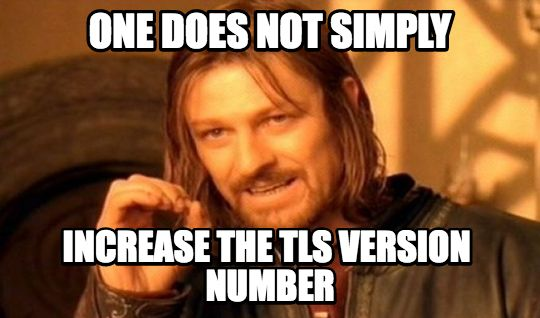
\includegraphics[width=4in]{932382}

\end{slide}

\begin{slide}
\heading{Alternate Proposal}

\begin{itemize}
\item Keep \verb^ClientHello^ version number at {3, 3} (TLS 1.2)

\item Introduce a new tls\_version extension
  \begin{itemize}
  \item Semantic is: a list of all supported versions
  \item Example: \verb^[ [3, 2], [3, 3], [3, 4], [53, 100] ]^
  \end{itemize}

\item ServerHello contains the negotiated version
\item All future versions negotiated this way
\begin{itemize}
\item Can fuzz for futureproofing
\end{itemize}

\item Discuss
\end{itemize}

\end{slide}


\begin{slide}
\heading{PSK and Client Auth}

\vspace{-4ex}
\begin{itemize}
\item Draft implies support for client authentication even with PSK mode
  \begin{itemize}
  \item Server just sends CertificateRequest
  \item Semantics of this are odd.
  \item 0-RTT is even worse
  \end{itemize}

\item Main proposal
  \begin{itemize}
  \item CertificateRequest not allowed when using PSK
  \item Use post-handshake client auth if you want this
  \end{itemize}

\item Fallback proposal
  \begin{itemize}
  \item PSK client auth needs an identity that is ``morally the same''
  \item Then clients can refuse to refresh
  \end{itemize}

\item Proposed resolution: ban client auth PSK
\end{itemize}

\end{slide}


\begin{slide}
\heading{Resumption Contexts and 0-RTT Finished}

\begin{itemize}
\item From the 0-RTT Finished:
\begin{itemize}
\item Proof of at least partial liveness of the PSK [via ticket age]
\item An integrity check for the information in the ClientHello
\end{itemize}
\item From the resumption context:
\begin{itemize}
\item Tie the context from the PSK-establishing connection to
  future handshakes.
\end{itemize}

\item Issues
  \begin{itemize}
  \item ``0'' resumption\_context for out-of-band PSK is problematic
  \item 
  \end{itemize}
\end{itemize}

\end{slide}



\begin{slide}
\heading{Interop Status}

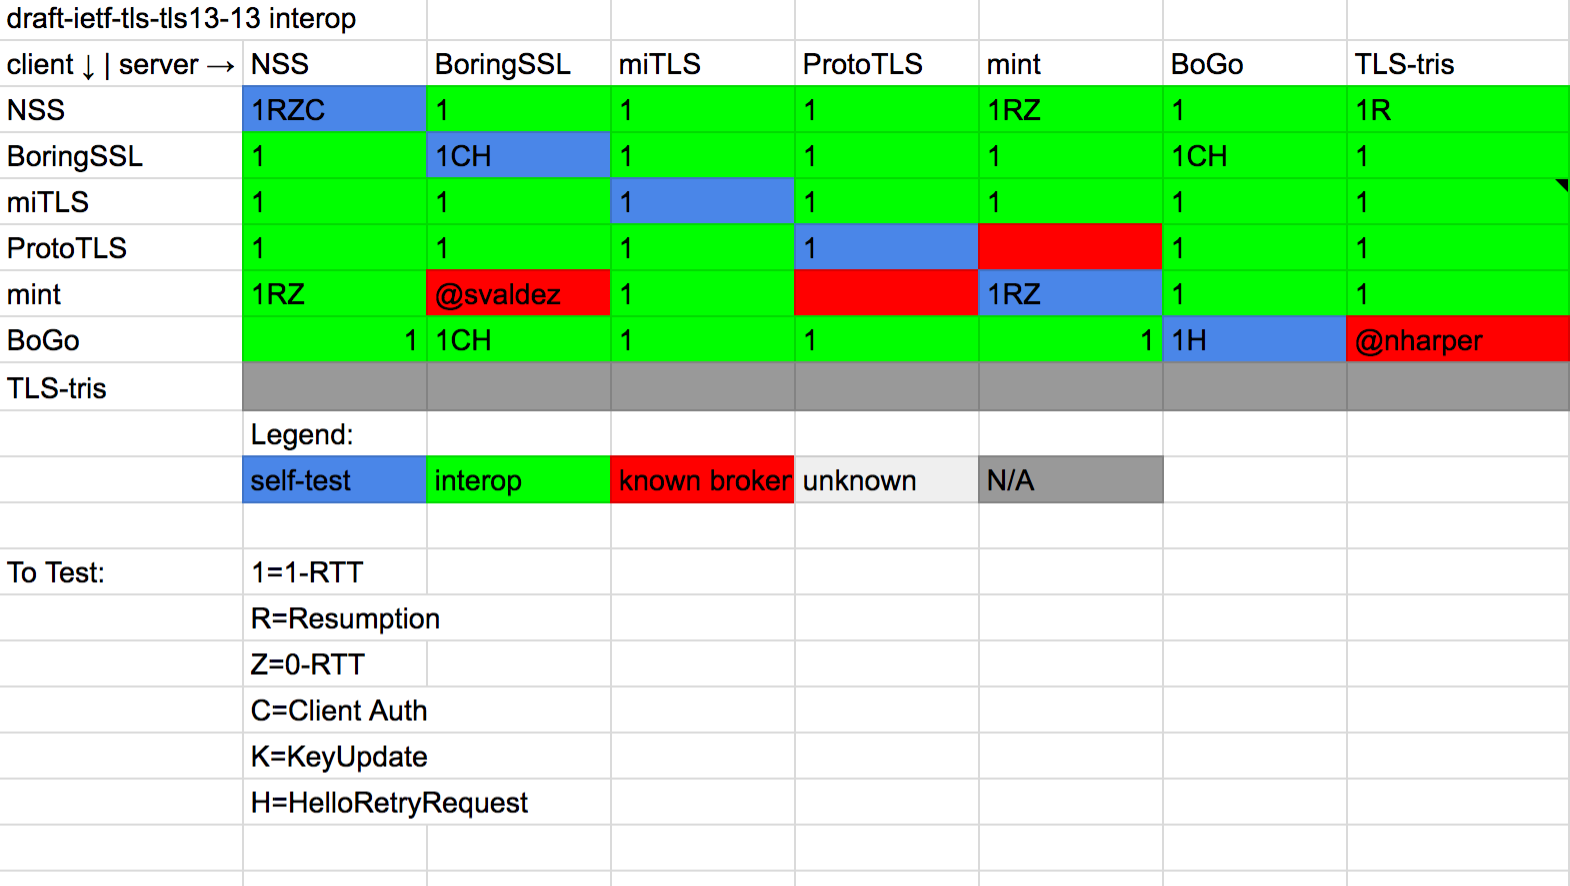
\includegraphics[width=4in]{interop-matrix}

\end{slide}


\begin{slide}
\heading{Timeline: Option \#1 (No big changes)}

\begin{tabular}{l l}
Aug 8th & draft-15: Wire format frozen (``Cryptographer's version'') \\
Aug 22nd & Implementations of draft-15 \\
Aug 29th & draft-16: Revised based on feedback \\
Aug 29th & WGLC \\
Sep 30th & WGLC Ends \\
\end{tabular}

\end{slide}


\begin{slide}
\heading{Timeline: Option \#2 (Change Negotiation or 0-RTT Finished)}

\begin{tabular}{l l}
Aug 8th & draft-15: Changes agreed at IETF 96 \\
Aug 22nd & Implementations of draft-15 \\
Aug 29th & draft-16: Revised; Wire format frozen (``cryptographer's version'')\\
Sep 12th & Implementations of draft-16 \\
Sep 19th & draft-17: Revised based on feedback \\
Sep 19th & WGLC \\
Oct 17th & WGLC Ends \\
\end{tabular}

\end{slide}


\end{document} 

                